

\subsection{3D Axis Configuration}
This section described keys which are used to configure the appearance of three dimensional figures. Some of them apply for two--dimensional plots as special case as well, and they will also be discussed in the respective sections of this manual.

\subsubsection{View Configuration}
\begin{pgfplotskey}{view=\marg{azimuth}\marg{elevation} (initially \{25\}\{30\})}
	Changes both view angles of a 3D axis. The azimuth (first argument) is the horizontal angle which is rotated around the $z$ axis. For a 3D plot, the $z$ axis always points to the top. The elevation (second argument) is the vertical rotation around the (rotated) $x$ axis. Positive elevation values indicate a view from above, negative a view from below. All values are measured in degree.

\pgfplotsexpensiveexample
\begin{codeexample}[]
\begin{tikzpicture}
	\begin{axis}[view={0}{0},
		xlabel=$x$,
		zlabel=$z$,
		title=View along the positive $y$ axis]
		\addplot3[surf] {x};
	\end{axis}
\end{tikzpicture}
\end{codeexample}

\pgfplotsexpensiveexample
\begin{codeexample}[]
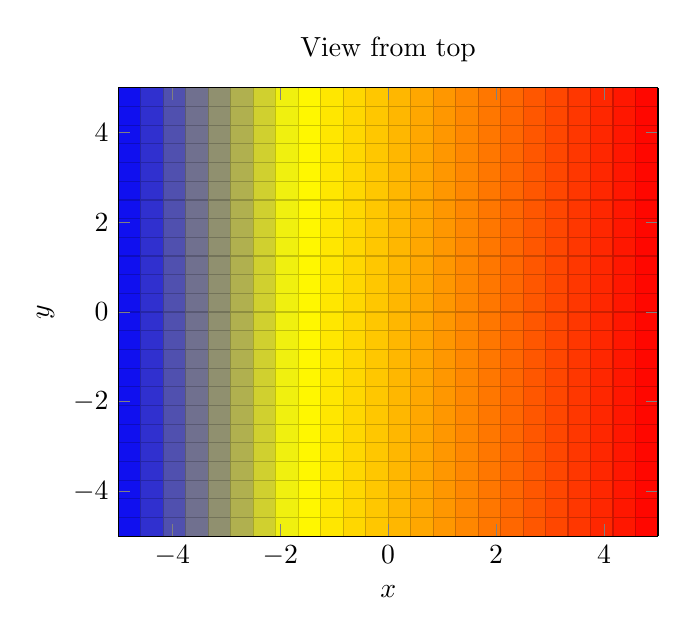
\begin{tikzpicture}
	\begin{axis}[view={0}{90},
		xlabel=$x$,
		ylabel=$y$,
		title=View from top]
		\addplot3[surf] {x};
	\end{axis}
\end{tikzpicture}
\end{codeexample}

\pgfplotsexpensiveexample
\begin{codeexample}[]
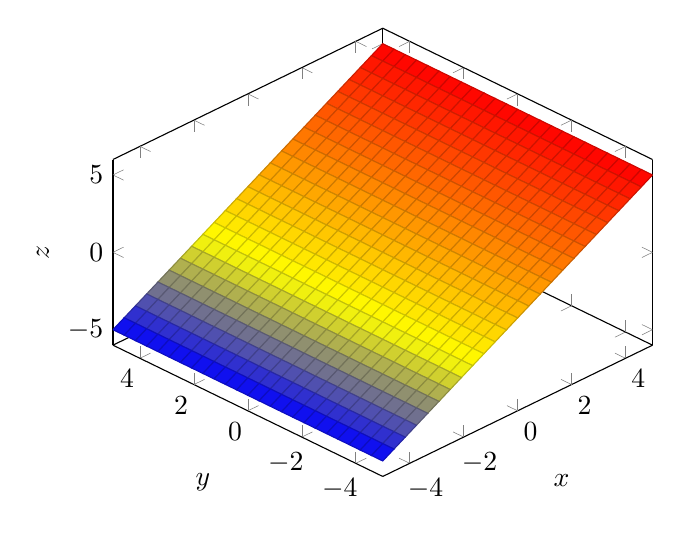
\begin{tikzpicture}
	\begin{axis}[view={-45}{45},
		xlabel=$x$,ylabel=$y$,zlabel=$z$]
		\addplot3[surf] {x};
	\end{axis}
\end{tikzpicture}
\end{codeexample}

	The |view| is computed as follows. The view is defined by two rotations: the first rotation uses the \meta{azimuth} angle to rotate around the $z$ axis. Afterwards, the view is rotated \meta{elevation} degrees around the \emph{rotated} $x$ axis (more precisely, it is rotated $-$\meta{elevation} degrees). The resulting transformed $x$--$z$--plane is the viewport, i.e.\ the view direction is always the transformed positive $y$ axis.

	The |view| argument is assignment compatible with matlab (tm), i.e.\ you can use 
	
	|[h,v] = view|
	
	\noindent in matlab and pack the resulting arguments into \PGFPlots\footnote{In case it does not work, try \texttt{h} and \texttt{-v} in \PGFPlots.}.

	If you work with |gnuplot|, you can convert the view arguments as follows: the |gnuplot| command

	|set view v,h|

	\noindent is \emph{equivalent} to |view={h}{90-v}|. For example, the default |gnuplot| configuration |set view 60,60| is equivalent to |view={60}{30}| in \PGFPlots.

	The |view| is (currently) always an orthogonal projection, no perspective is possible, yet.
\end{pgfplotskey}

\begin{pgfplotskeylist}{view/az=\marg{azimuth},view/h=\marg{azimuth} (initially 25)}
	Changes only the azimuth view angle, i.e.\ the horizontal (first) view angle which is rotated around the~$z$ axis.

\pgfplotsexpensiveexample
\begin{codeexample}[]
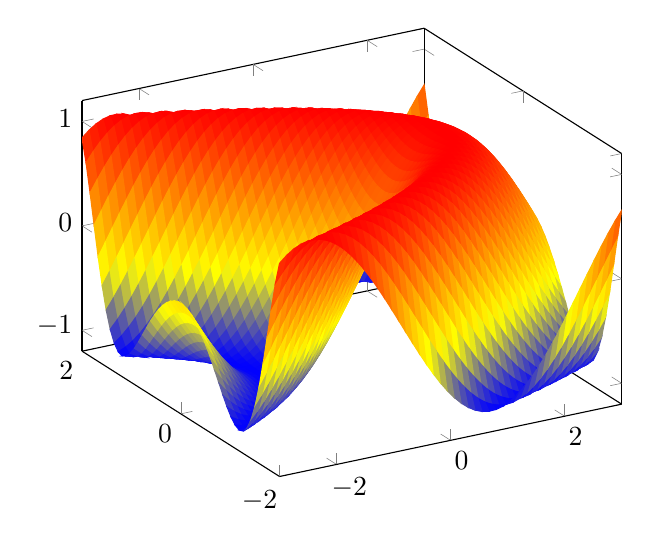
\begin{tikzpicture}
	\begin{axis}[view/h=-30]
	\addplot3[
		surf,
		%shader=interp,
		shader=flat,
		samples=50,
		domain=-3:3,y domain=-2:2] 
		{sin(deg(x+y^2))};
	\end{axis}
\end{tikzpicture}
\end{codeexample}

\pgfplotsexpensiveexample
\begin{codeexample}[]
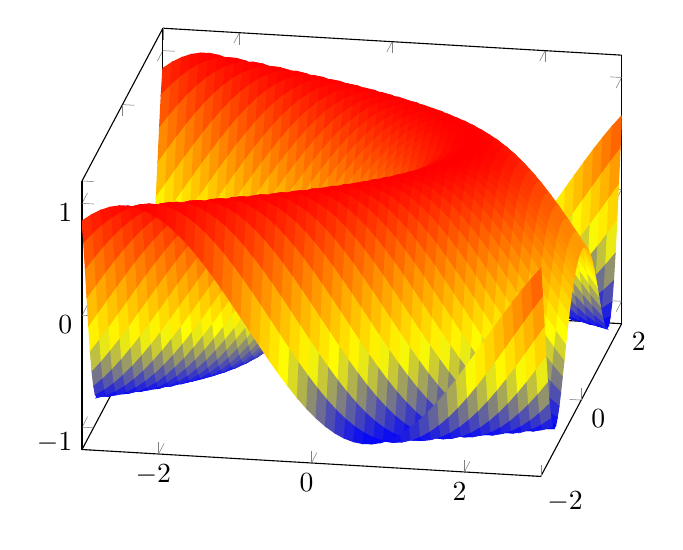
\begin{tikzpicture}
	\begin{axis}[view/h=10]
	\addplot3[
		surf,
		%shader=interp,
		shader=flat,
		samples=50,
		domain=-3:3,y domain=-2:2] 
		{sin(deg(x+y^2))};
	\end{axis}
\end{tikzpicture}
\end{codeexample}

\pgfplotsexpensiveexample
\begin{codeexample}[]
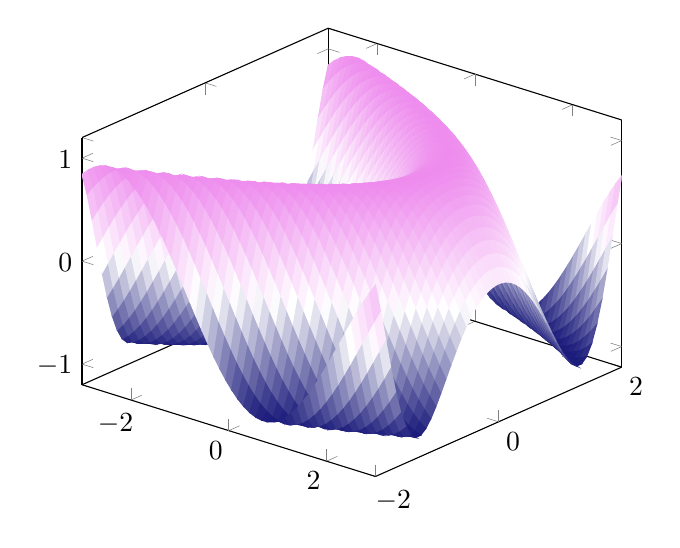
\begin{tikzpicture}
	\begin{axis}[view/h=40,colormap/violet]
	\addplot3[
		surf,
		%shader=interp,
		shader=flat,
		samples=50,
		domain=-3:3,y domain=-2:2] 
		{sin(deg(x+y^2))};
	\end{axis}
\end{tikzpicture}
\end{codeexample}

\pgfplotsexpensiveexample
\begin{codeexample}[]
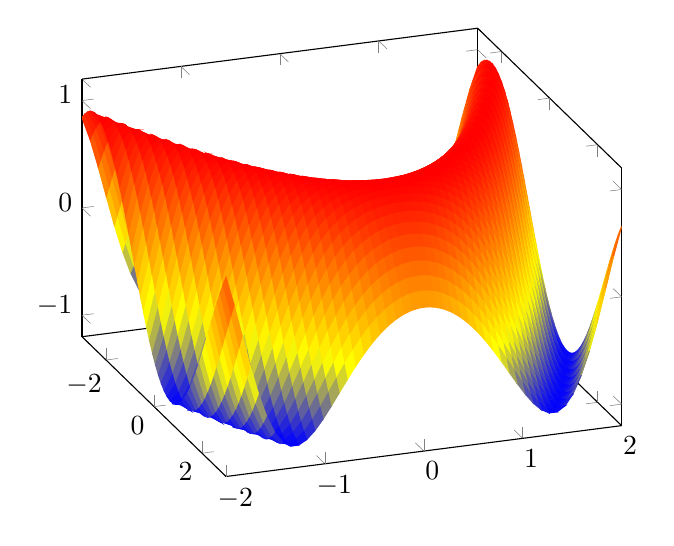
\begin{tikzpicture}
	\begin{axis}[view/h=70]
	\addplot3[
		surf,
		%shader=interp,
		shader=flat,
		samples=50,
		domain=-3:3,y domain=-2:2] 
		{sin(deg(x+y^2))};
	\end{axis}
\end{tikzpicture}
\end{codeexample}
\end{pgfplotskeylist}

\begin{pgfplotskeylist}{view/el=\marg{elevation},view/v=\marg{elevation} (initially 30)}
	Changes only the vertical elevation, i.e.\ the second argument to |view|. Positive values view from above, negative values from below. 
\end{pgfplotskeylist}

\subsubsection{Styles Used Only For 3D Axes}
\begin{stylekey}{/pgfplots/every 3d description}
	This style allows to change the appearance of \emph{descriptions} for three dimensional axes. Naturally, a three dimensional axis will display axis labels for $x$ and $y$ differently  than a two dimensional axis (for example, the $y$ axis label won't be rotated by 90 degrees). The |every 3d description| style installs the necessary display options for three dimensional axis descriptions.

	The initial value is:
\begin{codeexample}[code only]
\pgfkeys{
	/pgfplots/every 3d description/.style={
		% Only these description styles can be changed here:
		every axis x label/.style={at={(ticklabel cs:0.5)},
			anchor=near ticklabel},
		every axis y label/.style={at={(ticklabel cs:0.5)},
			anchor=near ticklabel},
		every x tick scale label/.style={
			at={(xticklabel cs:0.95,5pt)},
			anchor=near xticklabel,inner sep=0pt},
		every y tick scale label/.style={
			at={(yticklabel cs:0.95,5pt)},
			anchor=near yticklabel,inner sep=0pt},
		try min ticks=3,
	}%
}
\end{codeexample}

	As the name suggests, |every 3d description| can only be used to set styles for axis labels, tick labels and titles. It has \emph{not} been designed to reset other styles, you will need to change these options either for each axis separately or by means of user defined styles. The reason for this limitation is: other options can (and, in many cases) need to be set before the axis is processed. However, the decision whether we have a two dimensional or a three dimensional axis has to be postponed until the processing is more or less complete -- so only some remaining keys can be set.	
\end{stylekey}

\begin{stylekey}{/pgfplots/every 3d view \marg{h}\marg{v}}
	A style which can be used for fine tuning of the output for specific views.

	This style will be installed right after |every 3d description|, but before other axis description related keys are set (in other words: it has higher precedence than |every 3d description| but less precedence than keys provided to the axis directly).

	One example is preconfigured for |view={0}{90}| (from top):
\begin{codeexample}[code only]
\pgfplotsset{
	/pgfplots/every 3d view {0}{90}/.style={
		xlabel near ticks,
		ylabel near ticks,
		axis on top=true
	}
}
\end{codeexample}
\end{stylekey}


\subsubsection{Appearance Of The 3D Box}

\begin{pgfplotskey}{plot box ratio=\marg{x stretch}\marg{y stretch}\marg{z stretch} (initially {1}{1}{1})}
	Allows to customize the aspect ratio between the three different axes in a three dimensional plot.

	The |plot box ratio| is applied before any rotations and stretch--to--fill routines have been invoked. Thus, the initial setting |{1}{1}{1}| makes all axes equally long.

\pgfplotsexpensiveexample
\begin{codeexample}[]
\begin{tikzpicture}
\begin{axis}[
	view/h=60,
	plot box ratio={1}{1}{1},
	colormap={violet}{[1cm] rgb255(0cm)=(25,25,122)
		color(1cm)=(white) rgb255(5cm)=(238,140,238)},
	xlabel=$x$,
	ylabel=$t$,
	zlabel={$p(x,t)$},
	shader=faceted,
	title=Initial \texttt{plot box ratio},
]
	\addplot3[surf,y domain=0.02:3.5,samples=81]
		{1/(2*sqrt(pi*y)) * exp(0-x^2/y)};
	% the '0' is a work-around for a bug in PGF 2.00
\end{axis}
\end{tikzpicture}
\end{codeexample}

\pgfplotsexpensiveexample
\begin{codeexample}[]
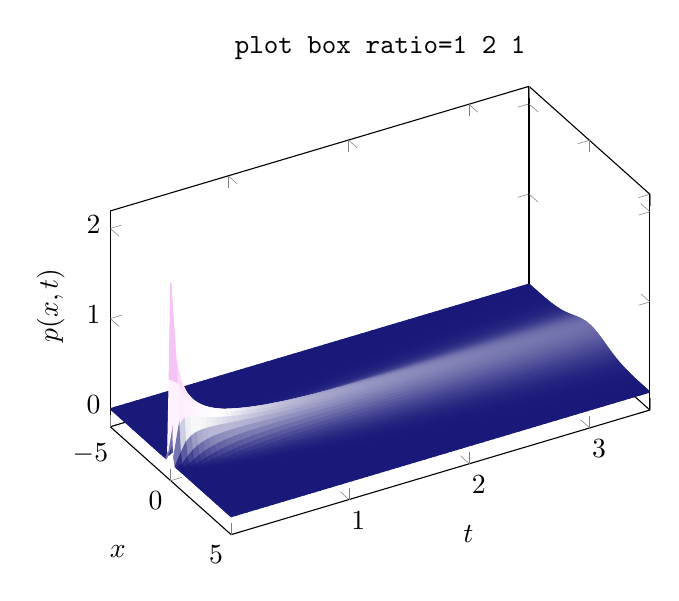
\begin{tikzpicture}
\begin{axis}[
	view/h=60,
	plot box ratio={1}{2}{1},
	colormap={violet}{[1cm] rgb255(0cm)=(25,25,122)
		color(1cm)=(white) rgb255(5cm)=(238,140,238)},
	xlabel=$x$,
	ylabel=$t$,
	zlabel={$p(x,t)$},
	shader=flat,
	title=\texttt{plot box ratio=1 2 1},
]
	\addplot3[surf,y domain=0.02:3.5,samples=81] 
		{1/(2*sqrt(pi*y)) * exp(0-x^2/y)};
	% the '0' is a work-around for a bug in PGF 2.00
\end{axis}
\end{tikzpicture}
\end{codeexample}

	This key applies only to three dimensional axes. After the scaling, the axes will be stretched to fill the |width| and |height| for this plot. Thus, the effects of |plot box ratio| might be undone by this stretching for particular views.
\end{pgfplotskey}


\begin{pgfplotskey}{3d box=\mchoice{background,complete,complete*} (initially background)}
	\label{pgfplots:key:3dbox}
	Allows to configure the appearance of boxed three dimensional axes.

	Type only |3d box| (without value) as alias for |3d box=complete|.

	The choice \declaretext{background} is the initial setting, it does not draw axis lines (and grid lines) which are in the foreground.
\begin{codeexample}[]
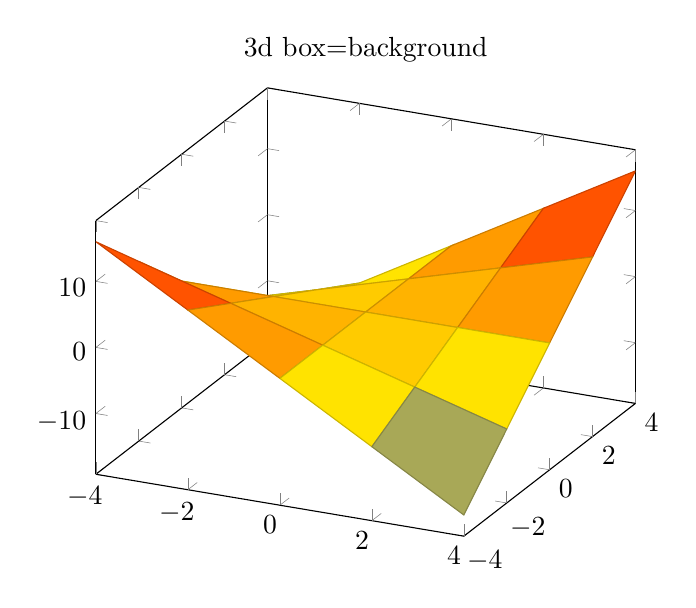
\begin{tikzpicture}
	\begin{axis}[
		3d box=background,
		% pretty printing, but irrelevant:
		title={3d box=background},
		samples=5,
		domain=-4:4,
		xtick=data,
		ytick=data,
	]
		\addplot3[surf] {x*y};
	\end{axis}
\end{tikzpicture}
\end{codeexample}

	The choice \declaretext{complete} also draws axis lines and tick lines in the foreground, but it doesn't draw grid lines in the foreground. The result yields a complete box:
\begin{codeexample}[]
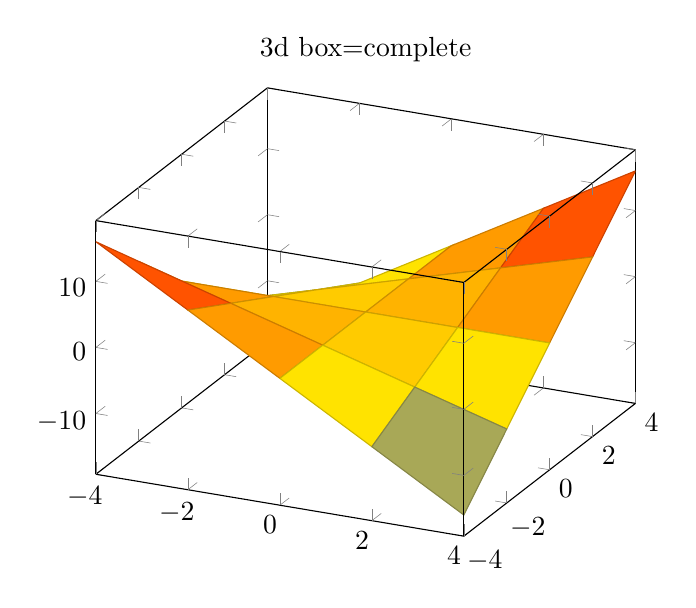
\begin{tikzpicture}
	\begin{axis}[
		3d box,% same as 3d box=complete
		% pretty printing, but irrelevant:
		title={3d box=complete},
		samples=5,
		domain=-4:4,
		xtick=data,
		ytick=data,
	]
		\addplot3[surf] {x*y};
	\end{axis}
\end{tikzpicture}
\end{codeexample}

	Finally, the choice \declaretext{complete*} is the same as |complete|, but it also draws grid lines.
\begin{codeexample}[]
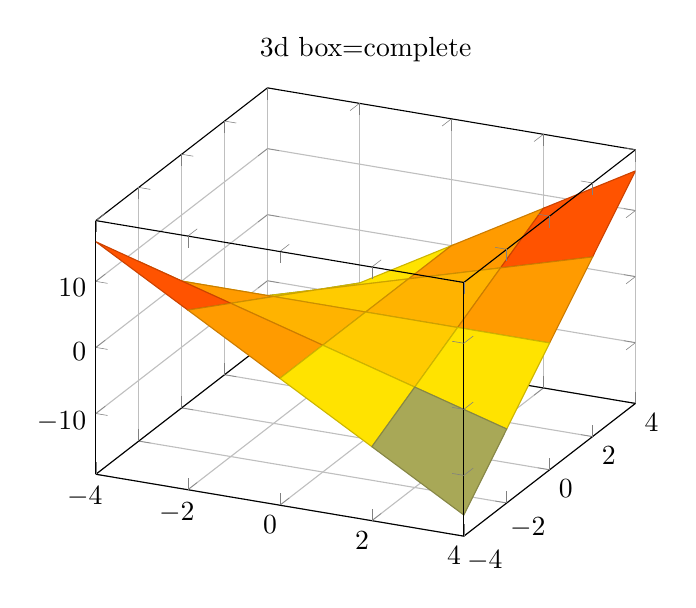
\begin{tikzpicture}
	\begin{axis}[
		3d box=complete,
		grid=major,
		title={3d box=complete},
		samples=5, domain=-4:4,
		xtick=data, ytick=data,
	]
		\addplot3[surf] {x*y};
	\end{axis}
\end{tikzpicture}%
~
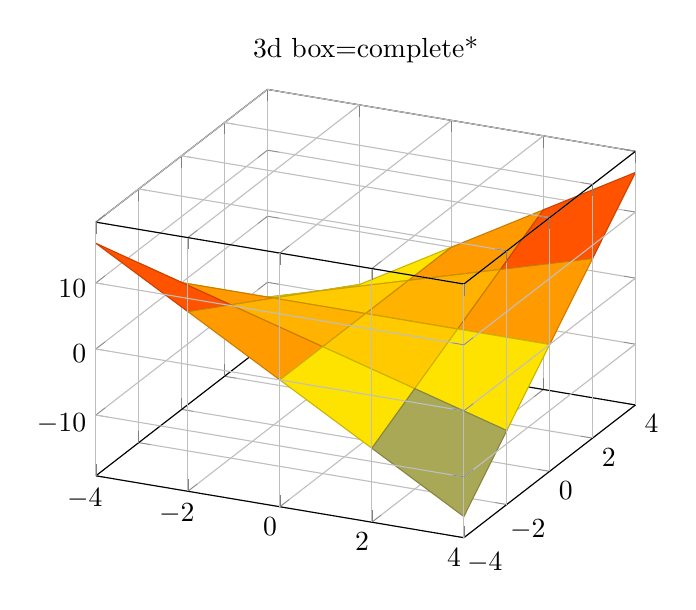
\begin{tikzpicture}
	\begin{axis}[
		3d box=complete*,
		grid=major,
		title={3d box=complete*},
		samples=5, domain=-4:4,
		xtick=data, ytick=data,
	]
		\addplot3[surf] {x*y};
	\end{axis}
\end{tikzpicture}
\end{codeexample}
	
	Before any foreground parts are actually processed, the style |every 3d box foreground| will be installed. This allows to change the appearance of foreground axis components like |tick style| or |axis line style| separately from the background components.

	Note that |3d box=complete| is \emph{only} available for boxed axes, i.e.\ together with |axis lines=box|. It is an error to use a different combination.
\end{pgfplotskey}



\subsubsection{Axis Line Variants}
\label{sec:pgfplots:axislines:3d}
Three dimensional axes also benefit from the |axis lines=box| or |axis lines=center| styles discussed in section~\ref{sec:pgfplots:axislines}. The choice |axis lines=box| is standard, it draws a box (probably affected by the |3d box=complete| key). 
The choice |axis lines=center| draws all three axes such that they pass through the origin. It might be necessary to combine this key with |axis on top| as there is no depth information.

\begin{codeexample}[]
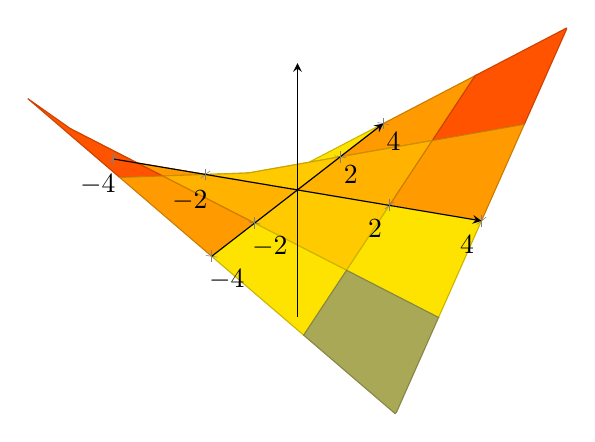
\begin{tikzpicture}
	\begin{axis}[
		axis lines=center,
		axis on top,
		samples=5, domain=-4:4,
		xtick=data, ytick=data,
		ztick=\empty, % no z ticks here
	]
		\addplot3[surf] {x*y};
	\end{axis}
\end{tikzpicture}
\end{codeexample}

The remaining choices |axis lines*=left| and |axis lines*=right| select different sets of axes in a way such that tick labels and axis label won't disturb the plot's content. The `|*|' suppress the use of special styles which are mainly adequate for 2d axes, see the documentation of |axis lines|. Such a set of axes is always on the boundary of the two--dimensional projection.  

The choice |axis lines*=left| chooses a set of axes which are left (or bottom, respectively) whereas the choice |axis lines*=right| chooses a set of axes which are on the right (or top, respectively):

\begin{codeexample}[]
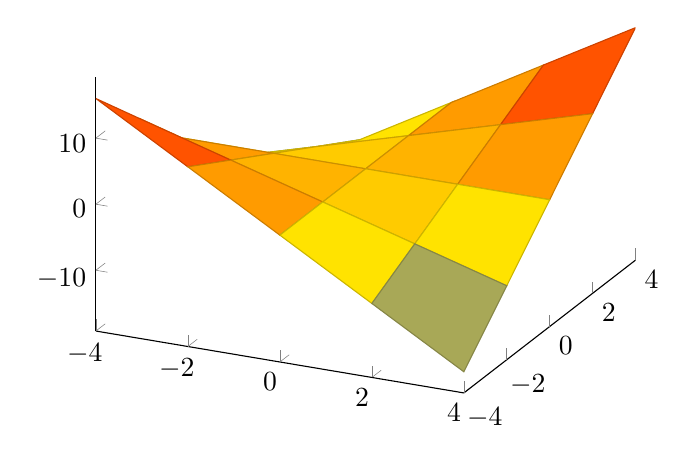
\begin{tikzpicture}
	\begin{axis}[
		axis lines*=left,
		samples=5, domain=-4:4,
		xtick=data, ytick=data,
	]
		\addplot3[surf] {x*y};
	\end{axis}
\end{tikzpicture}
\end{codeexample}

\begin{codeexample}[]
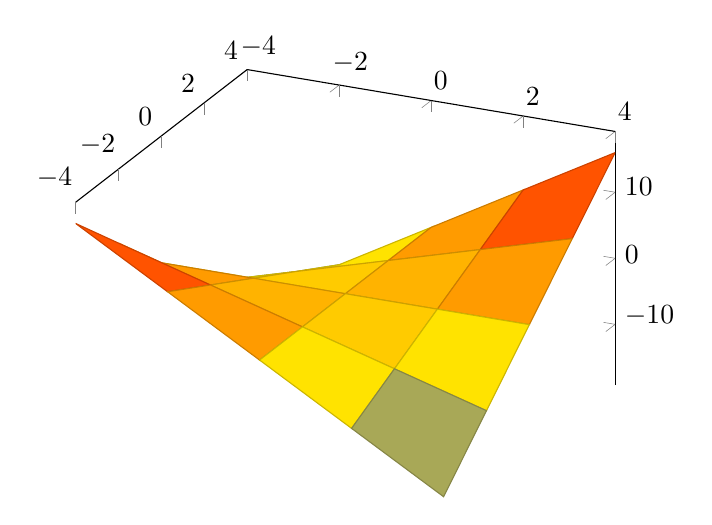
\begin{tikzpicture}
	\begin{axis}[
		axis lines*=right,
		samples=5, domain=-4:4,
		xtick=data, ytick=data,
	]
		\addplot3[surf] {x*y};
	\end{axis}
\end{tikzpicture}
\end{codeexample}

It is not (yet) possible to mix different styles like |axis x line=center,axis z line=top|.

